\documentclass{deimj}
\usepackage[dvipdfmx]{graphicx}
\usepackage[ipaex]{pxchfon}
\usepackage[hyphens]{url}
\usepackage{tabularx}
\usepackage{multirow}

% 印刷位置調整 %
% 必要に応じて値を変更してください.
\hoffset -10mm % <-- 左に 10mm 移動
\voffset -10mm % <-- 上に 10mm 移動

\newcommand{\AmSLaTeX}{%
$\mathcal A$\lower.4ex\hbox{$\!\mathcal M\!$}$\mathcal S$-\LaTeX}
\newcommand{\PS}{{\scshape Post\-Script}}
\def\BibTeX{{\rmfamily B\kern-.05em{\scshape i\kern-.025em b}\kern-.08em
T\kern-.1667em\lower.7ex\hbox{E}\kern-.125em X}}

\papernumber{DEIM Forum 2019 XX-Y}

% \jtitle{未訪問エリアの理解支援のための既訪問スポットに基づく類推情報提示手法}
\jtitle{ユーザの既訪問スポットの位置づけに基づく未訪問スポットの説明手法}
%\jsubtitle{サブタイトル} <- サブタイトルを付けたいときはこの行の先頭の % を取る
\authorlist{%
 \authorentry[em18011@ns.kogakuin.ac.jp]{潘 健太}{KENTA HAN}{UnivN}
 \authorentry[kitayama@cc.kogakuin.ac.jp]{北山 大輔}{DAISUGE KITAYAMA}{UnivN}
 }

\affiliate[UnivN]{工学院大学大学院工学研究科情報学専攻\hskip1zw
  〒163--8677 西新宿1-24-2}
 {School of Engineering,Kogakuin University\\
  1--24--2,Nisisinjyuku,Tokyo,163--8677 Japan}

\begin{document}
\pagestyle{empty}
\begin{jabstract}
近年,観光スポットを決める時にWeb上の観光情報を活用して計画を立てることが多くなっている.
しかし,ユーザが多くのエリアから訪問したいエリアを決めた上で,さらに自分のイメージに合う観光スポットを探すのは膨大な時間と労力を必要とする.
また,ユーザの未知なスポットに対する理解を支援するためには,既に訪問したことがある観光スポットの特徴を未訪問スポットにあてはめて理解を支援する説明手法を提案する.
本研究では,まず,観光スポットのユーザレビューを用いて特徴ベクトルを作成する.
次に,既に訪問したスポットと比較した差分ベクトルを用いて,観光スポットの独特な特徴を抽出する.
最後に,差分ベクトル間の類似度に基づいて既訪問スポットと未訪問スポットの関連付けし,その関係性を説明するためのキーワードを抽出する.
また,プロトタイプシステムを構築し,既訪問スポットと未訪問スポットとの説明情報の効果を検証する評価実験を行う.
\end{jabstract}

\begin{jkeyword}
観光スポット,理解支援,ユーザレビュー,分散表現
\end{jkeyword}
\maketitle

%%%%%%%%%%%%%%%%%%%%%%%%%%%%%%%%%%%%%%%%%%
%%%%%%%%%%%%%%%%%%%%%%%%%%%%%%%%%%%%%%%%%%
\section{はじめに}
\label{sec:はじめに}
旅行先を決定する時,旅行者は観光スポット検索サイトや観光情報に関連する書籍を見て観光スポットを選び,旅行計画を立てる.
しかし,ユーザにとって訪問したいエリアを決定した後,さらにエリア内に数多く存在する観光スポットから,自身のイメージから外れない観光スポットを見つけることは容易ではない.
行きたい観光スポットが決まっていない場合では,ランキングやおすすめ情報を見て観光スポットを決めることが多くなると考えられる.
Tripadvisor\footnote{https://www.tripadvisor.com/}やじゃらん\footnote{https://www.jalan.net/kankou/}などの観光スポット検索サイトでは,ユーザが特定の観光スポットを訪問した後レビューを投稿するため,観光スポットに関する豊富な情報がある.
しかし,ユーザは訪問したいエリアについての事前知識がないため,検索された観光スポットを1つずつ確認する必要がある.
よって,さまざまな観光スポットを効果的に理解するためには,既存の情報をもとにして,未知な情報と既知な情報との対応関係を考えることが不可欠となる.
この考え方は,以前に経験した事柄(ベースと呼ぶ)を,現在直面している事柄あるいは問題(ターゲットと呼ぶ)にあてはめる類推に相当する.
たとえば,金沢の「にし茶屋街」という未知なスポットに対して既訪問の京都の「花見小路」と似ていると説明するとイメージの理解がしやすくすることがある.

本研究では,ユーザの未訪問スポットに対する理解を支援するため,既に訪問したことがある観光スポットの特徴を未訪問スポットにあてはめて理解を支援する説明手法を提案する.
具体的には,ユーザは既に訪問したスポットおよび未訪問エリアを入力する.
そのとき,観光スポットのユーザレビューを用いて特徴ベクトルを作成する.
次に,既に訪問したスポットと比較した差分ベクトルを用いて,観光スポットの独特な特徴を抽出する.
最後に,差分ベクトル間の類似度に基づいて既訪問スポットと未訪問スポットの関連付けし,その関係性を説明するためのキーワードを抽出する.
このプロトタイプシステムにより,ユーザが未訪問スポットに対する理解の支援を目指す.図\ref{fig:Photo_Image}は提案手法の概念図である.

本論文の構成は下記のとおりである.
2章では,関連研究について述べる.
3章では,提案手法の概要について述べる.
4章では,構築したプロトタイプシステムの効果を検証する評価実験と考察について述べる.
最後に,5章では,まとめと今後の課題について述べる.

\begin{figure}[t]
  \begin{center}
    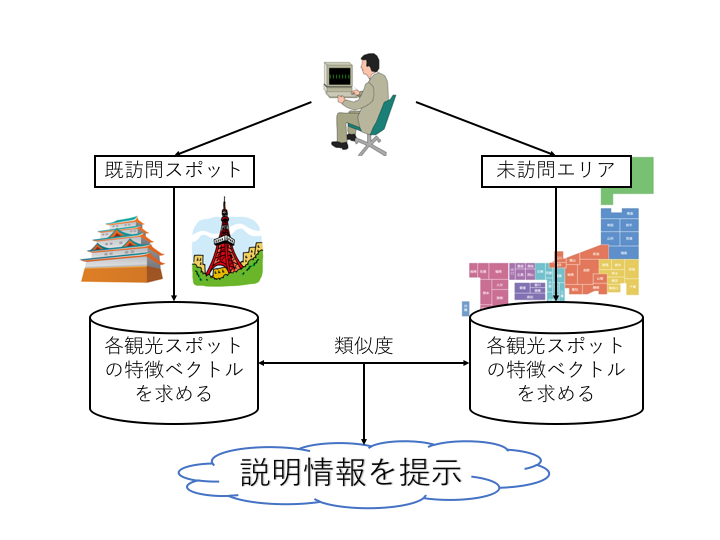
\includegraphics[clip,width=7.0cm]{picture/Photo_Image_jap.png}
    \caption{ユーザの既訪問スポットの位置づけに基づく未訪問スポット(エリア)の説明手法}
    \label{fig:Photo_Image}
   \end{center}
\end{figure}


%%%%%%%%%%%%%%%%%%%%%%%%%%%%%%%%%%%%%%%%%%
%%%%%%%%%%%%%%%%%%%%%%%%%%%%%%%%%%%%%%%%% 
\section{関連研究}
\label{sec:関連研究}
%%%%%%%%%%%%%%%%%%%%%%%%%%%%%%%%%%%%%%%%%%
\subsection{観光スポット検索と推薦システム}
ユーザの体験履歴を利用した検索や推薦システムに関する研究が数多く発表されている.
倉島ら\cite{Codd01}は,Flickrに投稿された写真のジオタグ情報を人々の旅行履歴として利用した旅行ルート推薦手法を提案した.
この手法では,ユーザの現在地から行きやすい場所とユーザの興味に合致した場所に移動しやすいと仮定し,行動モデルを生成している.
ユーザのジオタグ付き写真集合は,時間情報でソートすると個人の旅行履歴とみなすことができると考え,ジオタグ情報を利用してユーザの行動モデルを生成している.
北村らは\cite{Codd02},一般的な物体認識を用いて,過去の個人旅行写真から旅行計画のユーザの嗜好を推定することに基づいて観光地を推薦する方法を提案した.
物体認識システムを用いて,写真で撮った被写体情報のキーワードを取得し,グラフ視覚化技術によってキーワードの共起を表現した.
また,グラフの視覚化技術に基づいて旅行写真付きのグラフを視覚化するユーザインターフェイスを紹介した.
Chengらは\cite{Codd03},自由に利用できるコミュニティ寄稿の写真を活用して,パーソナライズされた旅行のおすすめに焦点を当て,特定のユーザープロファイルまたは属性を考慮し,パーソナライズされた旅行の推奨を行うことを提案した.

\subsection{類推とその応用}
類推は創造的思考に貢献すると指摘されてた\cite{Codd04}.
既知の知識(ベースと呼ぶ)から概念(ターゲットと呼ぶ)を獲得するときに類推思考が働くとされる\cite{Codd05}.
類推に関する研究の多くは,ベースとなる学習データとターゲットとなる問題が与えられ,物事の特徴を問題の特徴にマッピングして問題を解決するもの\cite{Codd06}である.
Gickらは,不確定な問題の解を見つけるためのガイドとして,異種ドメイン間の類推の使用を調査するように設計した.
学習データの与え方や機能について研究したもの\cite{Codd07}や,認知的な熟達度に応じて問題を解決するかどうかを明らかにしたもの\cite{Codd08}がある.
これらを含む従来研究の多くにおいては,類推に用いるベースとターゲットを与えたうえで,一定の手順に従って問題解決を行っている.
また,構造の類似性には3種類あり,特徴の共有数で決まる「対象レベルの類似性」,ベースに存在する関係とターゲットに存在する関係の共有度に基づく「関係レベルの類似性」,および題の解法あるいは目標レベルでの類似性である「プラグマティックな類似性」とがある\cite{Codd05},\cite{Codd09}.

従来のユーザの体験履歴を利用する手法では,履歴写真のジオタグ情報を分析し,ユーザの嗜好とする研究が多く行われている.
また,類推技術に関して学習支援でよくて使われている.
本研究では,既訪問スポットと未訪問スポットのレビューを使って,ユーザ既訪問スポット集合と未訪問スポット集合のそれぞれ集合の各スポットの相対的な特徴を求め,関連付けることによって,スポットに対する理解を支援するため説明情報を提示することができる.
また,本研究では,類推の質を明示的扱うため,構造の類似性「関係レベルの類似性」に近いと考えられる.

%%%%%%%%%%%%%%%%%%%%%%%%%%%%%%%%%%%%%%%%%%
%%%%%%%%%%%%%%%%%%%%%%%%%%%%%%%%%%%%%%%%%%
\section{未訪問スポットの説明手法}
\label{sec:未訪問スポットの説明手法}
我々は,ユーザの既訪問スポットの位置づけに基づく未訪問スポットの説明手法を提案する.
まず,ユーザが既に訪問した複数個の観光スポットと訪問したい観光スポットエリア情報を入力する.
本手法では,観光スポットのユーザレビューを用いて特徴ベクトルを生成する.
未訪問スポットも同様にエリア内の各スポットの特徴ベクトルを求める.
次に,既に訪問したスポットと比較した差分ベクトルを用いて,観光スポットの独特な特徴を抽出する.
未訪問スポットも同様にエリア内の各スポットの特徴ベクトルを求める.
差分ベクトル間の類似度に基づいて既訪問スポットと未訪問スポットの関連付ける.
最後に,その関係性を説明するためのキーワードを抽出する.

%%%%%%%%%%%%%%%%%%%%%%%%%%%%%%%%%%%%%%%%%%
\subsection{スポットのレビューから特徴ベクトル生成}
\label{subsec:スポットのレビューから特徴ベクトル生成}
本稿に置いて,レビューデータは2016年09月末までじゃらんから取得したものを用いる.
分散表現\cite{Codd10}を用いて観光スポットの特徴ベクトルの作成する.
そのとき,観光スポット毎のレビューをまとめて1つの文書として扱う.
本研究では,Pythonのライブラリであるgensim\footnote{https://radimrehurek.com/gensim/models/doc2vec.html}を使って,分散表現を計算する.
学習方法として,Distributed Bag-of-Wordsを利用して,各スポットの全レビューを使って300次元で作成したベクトルを使う.
既訪問スポットや未訪問スポットのレビューベクトルは,形態素解析器であるMeCab\cite{Codd11}を辞書「mecab-ipadic-NEologd」\footnote{https://github.com/neologd/mecab-ipadic-neologd/}使って,分かち書き(原型)したレビューを利用して作成する.

%%%%%%%%%%%%%%%%%%%%%%%%%%%%%%%%%%%%%%%%%%
\subsection{観光スポットの役割に関する相対的な特徴}
\label{subsec:観光スポットの役割に関する相対的な特徴}
\begin{figure}[t]
  \begin{center}
    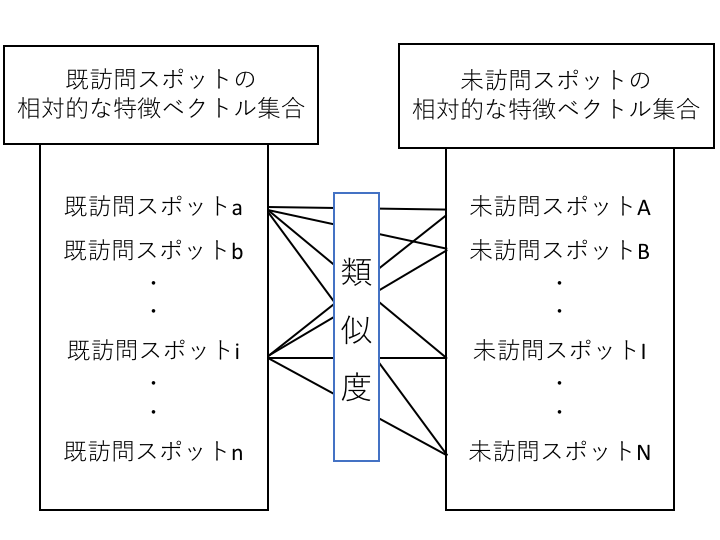
\includegraphics[clip,width=7.0cm]{picture/Photo_CosSim_jap.png}
    \caption{類似度計算概念図}
    \label{fig:Photo_CosSim}
  \end{center}
\end{figure}

本手法では,他の観光スポットと比較したとき相対的な特徴を用いて観光スポットの特徴を抽出する.
相対的な特徴とは,ターゲットである観光スポットが,ある観光スポット集合の平均的な特徴と比較した場合における独特な特徴と定義する.
たとえば,日本の有名な観光スポットの中に「東京都庁舎展望台」と「鹿苑寺」が存在する場合を考える.
このとき,「金閣寺」の相対的な特徴は,お寺,金色,京都などである.
一方,「東京都庁舎展望台」の相対的な特徴は,展望,夜景,建物,新宿などである.
さまざまな観光スポットと比較すると,相対的な特徴は一般的な特徴,カテゴリ,場所となる.

他の例として,京都の寺院の中に「金閣寺」と「清水寺」が存在する場合を考える.
このとき,「金閣寺」の相対的な特徴は,金色,金箔,輝きなどである.
一方,「清水寺」の相対的な特徴は,舞台や一望などである.
どちらも京都にある寺院であるため,京都や寺院に関連する特徴は相対的な特徴として表示されません.
その代わりに,より詳細な特徴が相対的な特徴として得られる.

相対的な特徴ベクトル$r_{state,i}$は,式\ref{math:Vector difference}として定義される.
相対的な特徴ベクトルは,そのスポット自体の特徴ベクトルから他のスポットの特徴ベクトルの平均を引いた値によって得られる.
$S_{state} =\{s_1,s_2,\dots,s_n\}$は,既訪問スポット集合や未訪問スポット集合となっている.
$state$は$'f'$のとき,既訪問スポット集合として定義する.
$state$は$'u'$のとき,未訪問スポット集合として定義する.
$s_i$は集合$S_{state}$内の観光スポットの特徴ベクトルを示している.

\begin{equation}
  r_{state,i}=s_i-average(S_{state}-s_i)
  \label{math:Vector difference}
\end{equation}

%%%%%%%%%%%%%%%%%%%%%%%%%%%%%%%%%%%%%%%%%%
\subsection{説明スポットの決定}
\label{subsec:説明スポットの決定}
未訪問エリア内のスポットは既訪問スポットを使って説明する.
したがって,未訪問スポットと既訪問スポットを,既訪問スポット$r_{f,i}$と未訪問スポット$r_{u,j}$の相対的な特徴ベクトルによって計算された類似度に基づいて関連付けを行う.(図\ref{fig:Photo_CosSim}).
類似度計算には,コサイン尺度(式\ref{math:CosSim})を用いる.
\begin{eqnarray}
  cos(r_{f,i},r_{u,j})=\frac{r_{f,i} \cdot r_{u,j}}{|r_{f,i}| \times |r_{u,j}|}
  \label{math:CosSim}
\end{eqnarray}

関連付け手順について説明する.
まず,特定のスポットに最も類似度が高いスポットと関連付ける.
このとき,類似度が閾値(本研究では0.125)以下である場合は関連付けを行わない.
また,未訪問スポットと類似度が最も高い既訪問スポットと関連付けられているか,既訪問スポットと類似度が最も高い未訪問スポットと関連付けられているかによって結果が異なる.

前者の方法では,すべての類似度が閾値を超えると,すべての既訪問スポットが対応するスポットがあるが,すべての未訪問スポットが対応するスポットがあるわけではない.
一方,後者の方法では,すべての類似度が閾値を超えると,すべての未訪問スポットが対応するスポットがある.
本手法では,未訪問スポットを説明するために後者の方法を採用する.

%%%%%%%%%%%%%%%%%%%%%%%%%%%%%%%%%%%%%%%%%%
\subsection{説明するための役割語の抽出}
\label{subsec:説明するための役割語の抽出}
未訪問スポットと既訪問スポットの関係性を表すため,ユーザにキーワードを提示する.
しかし,相対的な特徴ベクトルから単語の特徴を得ることはできないので,他の方法を使って単語を抽出する.

前提として,すべてのレビューは日本語の形態素解析器MeCabによって単語を分割する.
\ref{スポットのレビューから特徴ベクトル生成}節の``mecab-ipadic-NEologd''辞書を利用する.
しかし,助詞,助動詞,連体詞,記号,ストップワードを削除する(表\ref{table:mecab}).

\begin{table}[t]
  \caption{形態素解析の例}
  \label{table:mecab}
  \centering
    \begin{tabular}{c|p{23zw}} \hline
      レビュー文書 & 園内も広く,気分転換に散歩したりするのにちょうどよい.きれいに清掃などもされていて,気分がよいです.\\
      \hline
      形態素解析 & 園内 広い 気分転換 散歩 ちょうど よい きれい 清掃 気分 よい\\
      \hline
    \end{tabular}
\end{table}

キーワード抽出手順について説明する.
まず,TFIDF法を使って対象となる既訪問スポットと未訪問スポットの特徴語とTFIDF値を取得する.
次に,2つのスポットの共通する特徴語のスコアとしてTFIDF値の調和平均を計算する.
最後に,スコアが高い特徴語を説明可能な単語として抽出する.

スポット内のキーワード特徴値は,式\ref{math:TFIDF}で定義する.
\begin{equation}
  TFIDF(t,d,state) = TF(t,d) \times log\Biggr(\frac{|S_{state}|}{DF(t,state)}\Biggr)
  \label{math:TFIDF}
\end{equation}

$TF(t,d)$は,文書$d$においてのキーワード$t$の数である.
$d$は,スポットのすべてのレビューを1つにまとめた文書である.
$DF(t,state)$は,キーワード$t$を含む文書の数である.
$|S_{state}|$はスポットの総数である.
$state$が$f$の場合,ユーザが入力した既訪問スポット集合を使用してTFIDF値を計算する.
$state$が$u$の場合,ユーザが入力したエリアに含まれている未訪問スポット集合を使用してTFIDF値を計算する.

2つのスポットに共通する特徴語のTFIDF値の調和平均を用いて,関連付けした既訪問スポットと未訪問スポットの説明可能なキーワードを抽出する.
まず,既訪問スポットと未訪問スポットのレビュー文書でよく出現する単語を抽出する.
次に,抽出した単語のスコアは式\ref{math:Harmonic Mean}によって定義する.
$TFIDF(t,d,f)$と$TFIDF(t,d,u)$は同じ単語がそれぞれ既訪問スポットのTFIDF値と未訪問スポットのTFIDF値を示している.
単語スコアの値が大きいのとき,その単語は各スポットにおいて重要度が高いことを示している.
よって,単語スコアの上位$N$個の単語が説明情報としてユーザに提示する(図\ref{fig:Photo_Map}).

\begin{eqnarray}
  score(t,d) = \frac{2 \times TFIDF(t,d,f) \times TFIDF(t,d,u)}{TFIDF(t,d,f) + TFIDF(t,d,u)}
  \label{math:Harmonic Mean}
\end{eqnarray}

\begin{figure}[t]
  \begin{center}
    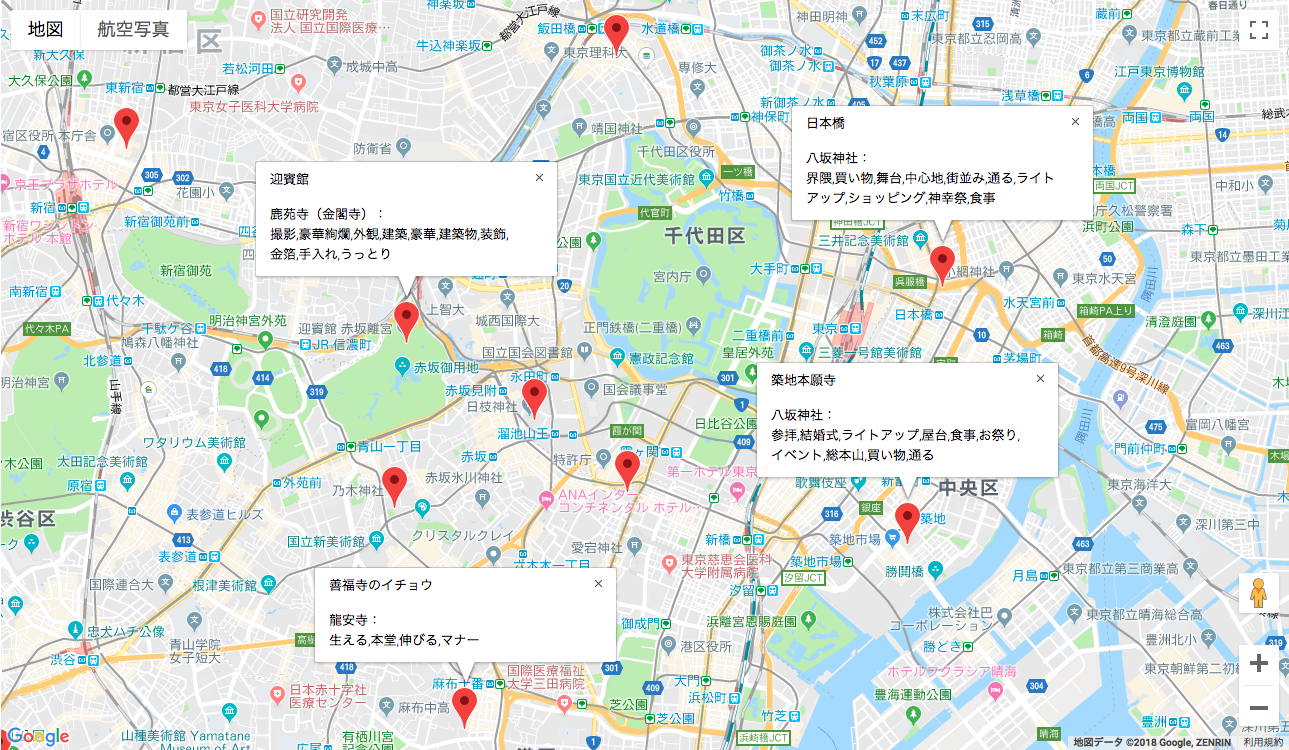
\includegraphics[clip,width=8.0cm]{picture/Photo_Map.png}
    \caption{プロトタイプシステムのユーザインターフェース}
    \label{fig:Photo_Map}
   \end{center}
\end{figure}

%%%%%%%%%%%%%%%%%%%%%%%%%%%%%%%%%%%%%%%%%%
\subsection{未訪問スポットの説明情報の例}
\label{subsec:未訪問スポットの説明情報の例}

\begin{table}[t]
  \caption{既訪問スポット集合と未訪問スポット集合}
  \label{table:既訪問スポット集合と未訪問スポット集合}
  \centering
  \begin{tabular}{l|l}
  \hline
  \multicolumn{1}{c|}{既訪問スポット名} & \multicolumn{1}{c}{未訪問スポット名} \\ \hline
  浅草寺                           & 東京ディズニーランド(R)                \\
  小田原城址公園                       & 新宿御苑                         \\
  伏見稲荷大社                        & 東京スカイツリー                     \\
  奈良公園                          & 東京タワー大展望台                    \\
  三島スカイウォーク                     & 明治神宮                         \\ \hline
  \end{tabular}
\end{table}

\begin{table*}[t]
  \caption{説明情報の例}
  \label{table:説明情報の例}
  \centering
  \begin{tabular}{l|l|l}
  \hline
  \multicolumn{1}{c|}{未訪問スポット} & \multicolumn{1}{c|}{既訪問スポット} & \multicolumn{1}{c}{説明情報}                     \\ \hline
  新宿御苑                      & 小田原城址公園                         & お花見,咲き誇る,園内,桜の時,のんびり,手入れ,自然,遊具,ツツジ          \\
  東京スカイツリー                     & 三島スカイウォーク                    & 富士山,揺れ,高所恐怖症,揺れる,天井,絶景,エレベーター,パノラマ,展望デッキ,昇る \\ \hline
  \end{tabular}
\end{table*}

表\ref{table:既訪問スポット集合と未訪問スポット集合}は,ユーザが既に訪問したことがあるスポットと,未訪問スポットの集合の例を示している.
未訪問スポットは東京都内からランダムに選んだ5つのスポットである.
表\ref{table:説明情報の例}は,\ref{sec:未訪問スポットの説明手法}節で提案して方法を用いて説明可能な単語の結果を示している.

公園という特徴に注目すると,未訪問スポット集合の中で公園に最も近いスポットは「新宿御苑」であると考えられる.
既訪問スポット集合の中には,「小田原城址公園」と「奈良公園」の2つの公園がある.
「小田原城址公園」には花や遊具に対する記述が多く,「奈良公園」には鹿や草に対する記述が多い.
「新宿御苑」には花や遊具に対する記述が多いため,「小田原城址公園」との関係性があると考えられる.

「三島スカイウォーク」は既訪問スポット集合の中で眺めがいい,高いの特徴が最も強いことが考えられる.
一方,未訪問スポット集合の中で眺めがいい,高いの特徴が強いのは「東京スカイツリー」や「東京タワー大展望台」の2つがある.
このとき,どちらも正しい回答だと思う.
この例では,「東京スカイツリー」はより見やすいと考えられるため関連付けされる.
また,説明キーワードとして「富士山」が抽出される.
良い景色を強調する言葉として一般的であり,これによって関係を適切に表現している.
提案手法の方は各関係の特徴を示すことができる.

%%%%%%%%%%%%%%%%%%%%%%%%%%%%%%%%%%%%%%%%%%
%%%%%%%%%%%%%%%%%%%%%%%%%%%%%%%%%%%%%%%%%%
\section{評価実験}
\label{sec:評価実験}
%%%%%%%%%%%%%%%%%%%%%%%%%%%%%%%%%%%%%%%%%%
\subsection{実験内容}
提案手法を他の手法と比較して評価を行う.
以下の3つの方法を使って比較する.
\begin{description}
  \item A.メタデータ(カテゴリ,滞在時間,訪問時期)
  \item B.分散表現(特徴ベクトル)
  \item C.提案手法(相対的な特徴ベクトル)
\end{description}

方法Aは,観光スポット検索サイトでスポットを検索するためのメタデータである.
次のように,検索によく使われる3つのメタデータを選択する.
\begin{itemize}
 \item カテゴリ:神社・神宮・寺院,観光施設・名所巡り等
 \item 滞在時間:1時間未満,1\verb|~|2時間等
 \item 訪問時期:1\verb|~|12月,春,夏,秋,冬
\end{itemize}

方法Aでは,同じカテゴリ,同じ滞在時間,同じ季節の既訪問スポットと未訪問スポットを抽出する.
抽出できない場合は,季節,滞在時間,カテゴリの順に情報を削除している.
未訪問スポットが複数ある場合は,レビュー数が最も多いスポットを選択する.
最後に,\ref{subsec:説明するための役割語の抽出}節を用いて説明可能な単語を抽出し,被験者に提示する.

方法Bでは,各スポットの特徴として\ref{subsec:スポットのレビューから特徴ベクトル生成}節で作成された特徴ベクトルを使用する.
そして,\ref{subsec:説明するための役割語の抽出}節を用いて説明可能な単語を抽出し,被験者に提示する.

クラウドソーシングのサービスである,CrowdWorks\footnote{https://crowdworks.jp/}を利用して24人の被験者を集めた.
各方法を用いて,被験者の既訪問スポットに基づいて,未訪問スポットの説明可能な情報を提示した.
まず,被験者は自分が既に訪れたことのある観光スポットを入力した.
被験者は4から10個のスポットを入力すると指示した.
本実験では,入力文字列とシステム内のスポット名と照会するために,入力文字列と同様にスポット名候補の中から対象スポットを選択した.
次に,被験者は旅行などに行ったことがなく,これから訪れたい都道府県を入力した.
関連付けした既訪問スポットと未訪問スポット,および方法Aから方法Cとそれぞれの説明可能なキーワードを提示した.
キーワードは最大5つを提示した(N = 5).
結果を評価するために,被験者は以下の5つの選択肢から1つを選んでもらった.
\begin{enumerate}
  \item キーワードなし.
  \item 2つのスポットにそもそも関係性があるが,キーワードにより関係が明確になった.
  \item 2つのスポットの関係にキーワードにより初めて気がついた.
  \item 2つのスポットに関係性があるがキーワードは関係性を表していない.
  \item 2つのスポットに関係性はない.
\end{enumerate}

%%%%%%%%%%%%%%%%%%%%%%%%%%%%%%%%%%%%%%%%%%
\subsection{実験結果と考察}
\label{subsec:実験結果}
\begin{table}[t]
  \caption{実験結果}
  \label{table:実験結果}
  \centering
  \begin{tabular}{c|r|r|r|r}
  \hline
  評価 & \multicolumn{1}{c|}{方法A} & \multicolumn{1}{c|}{方法B} & \multicolumn{1}{c|}{方法C} &  \multicolumn{1}{c}{合計} \\ \hline
  1  & 0                      & 0                      & 0                       & 0                      \\
  2  & 19                     & 44                     & 32                     & 95                    \\
  3  & 20                     & 62                     & 53                      & 135                    \\
  4  & 1                      & 3                      & 3                      & 7                     \\
  5  & 6                      & 21                     & 21                     & 48                     \\\hline
  合計 & 46                     & 130                    & 109                    & 285                    \\ \hline
  \end{tabular}
\end{table}

表\ref{table:実験結果}は方法Aから方法Cの各実験結果の数を示している.
評価実験では,使用可能のデータの合計は285である.
方法Aは,未訪問スポットに関連する既訪問スポットの数が最も少ない.
方法Bは,未訪問スポットに関連する既訪問スポットの数が最も多い.

\begin{table}[t]
  \caption{説明情報における評価の割合}
  \label{table:説明情報における評価の割合}
  \centering
  \begin{tabular}{c|r|r|r}
  \hline
  評価 & \multicolumn{1}{c|}{方法A} & \multicolumn{1}{c|}{方法B} & \multicolumn{1}{c}{方法C} \\ \hline
  1  & 0.00\%                     & 0.00\%                     & 0.00\% \\
  2  & 41.30\%                    & 33.85\%                    & 29.36\% \\
  3  & 43.48\%                    & 47.69\%                    & 48.62\% \\
  4  & 2.17\%                     & 2.31\%                     & 2.75\% \\
  5  & 13.04\%                    & 16.15\%                    & 19.27\% \\ \hline
  \end{tabular}
\end{table}

\begin{table}[t]
  \caption{既訪問スポットのカテゴリが異なる場合と類似する場合の評価の割合}
  \label{table:既訪問スポットのカテゴリが異なる場合と類似する場合の評価の割合}
  \centering
  \begin{tabular}{c|r|r}
  \hline
  & \multicolumn{1}{c|}{\begin{tabular}[c]{@{}c@{}}既訪問スポットが\\ 異なる場合\end{tabular}} & \multicolumn{1}{c}{\begin{tabular}[c]{@{}c@{}}既訪問スポットが\\ 類似する場合\end{tabular}} \\ \hline
  説明情報B\&評価1 & 56.82\%                            & 43.18\%                            \\
  説明情報C\&評価1 & 71.87\%                            & 28.13\%                            \\ \hline
  説明情報B\&評価2 & 51.61\%                            & 48.39\%                            \\
  説明情報C\&評価2 & 52.83\%                            & 47.170\%                            \\ \hline
\end{tabular}
\end{table}

表\ref{table:説明情報における評価の割合}は,方法AからCにおける選択肢1から5としての実験結果の数の割合を示している.
方法Aについて,多くの被験者が選択肢のNo.2を選している.
このことから,方法Aは明らかな関係にあるスポット同士を関連付けることができることがわかった.
他の方法と比較して,方法C(提案手法)では,選択肢No.2の割合が減少し,選択肢No.3の割合が増加している.
このことから,方法Cは隠れた関係を見つけて被験者に提示することができると考えた.
しかし,選択肢N0.5の割合も増加しているため,無関係なスポットを抽出しやすくなったといえる.

選択肢2と3を合計すると,方法Aが最も高くなった.
このことから,説明するためのスポットの関連付けの精度が最も高いといえる.
しかし,上述のように,選択肢2の意味は自然な関係であり,方法Aは少数しか抽出することができない.
我々にとって,選択肢2と3はトレードオフの関係にあることが考えられている.
選択肢2は説明する必要がない関係であり,選択肢3は説明に値する関係である.
選択肢2を維持しながら,選択肢3をできるだけ増やすことが重要だけ思う.
この観点からも,方法Bと提案手法は同程度の精度を示していると考えられる.

選択肢3は,キーワードの抽出に失敗した場合に選択肢5になる可能性が高いと考えられる.
したがって,キーワード抽出方法を改善する必要がある.

方法Bと方法Cについては,被験者が入力した既訪問スポットのカテゴリが異なる場合も同様で,選択肢2と選択肢3の評価の割合は表\ref{table:既訪問スポットのカテゴリが異なる場合と類似する場合の評価の割合}である.
提案手法である方法Cを使用すると,被験者が既訪問スポットと関係なしで,被験者に有意味なキーワードを提示することができる.
相対的な特徴ベクトルを用いることによって,カテゴリに渡って各スポットの特徴を求めることができるといえる.
既訪問スポットのジャンルが類似する場合では,方法Bの方かより良い評価となっている.

%%%%%%%%%%%%%%%%%%%%%%%%%%%%%%%%%%%%%%%%%%
%%%%%%%%%%%%%%%%%%%%%%%%%%%%%%%%%%%%%%%%%%
\section{まとめと今後の課題}
\label{sec:まとめと今後の課題}

本研究では,ユーザが行きたい観光スポットが決まっていない場合,ランキング,おすすめ情報やカテゴリなどに観光検索情報を使用することによって,検索した観光スポットがに対する理解が困難であることを着目した.
未訪問スポットに対する理解を支援するために,理解が困難の点をユーザが既に訪れたことがあるスポットと比較することによって,理解を支援する説明手法を提案した.

評価実験では,3つの説明方法を用いて比較を行った.
結果として,カテゴリを利用する場合では,未訪問スポットと関係する既訪問スポットが最も少ない.
相対的な特徴ベクトルと調和平均を利用することによって,各スポットの特徴を求めることができる.
また,意外性がある未訪問スポットと既訪問スポットを関連付けることができ,ユーザが知らない観光スポットに対する興味と関心を集めることができる可能性があることを確認した.

今後の課題としては,実験時に得られたユーザに提示するキーワード,未訪問スポットと既訪問スポットのカテゴリの関連性を分析する.
また,ユーザに提示する各キーワードの有効性と関係性についての評価を行う予定である.

今後の課題としては,実験時に得られたユーザに提示するキーワード間の関連性を分析する.
また,ユーザに提示する各キーワードの有効性と関連性についての評価を行う予定である.

%%%%%%%%%%%%%%%%%%%%%%%%%%%%%%%%%%%%%%%%%%
\section*{謝辞}
%%%%%%%%%%%%%%%%%%%%%%%%%%%%%%%%%%%%%%%%%%
% 本研究の一部は,平成29年度科研費若手研究(B)(課題番号:15K16091),および挑戦的萌芽研究(課題番号:16K12536)によるものです.ここに記して謝意を表すものとします.


%%%%%%%%%%%%%%%%%%%%%%%%%%%%%%%%%%%%%%%%%%
% 文献 Reference
%%%%%%%%%%%%%%%%%%%%%%%%%%%%%%%%%%%%%%%%%%
%\vspace{30mm} <- 文献が本文と近すぎるときは適宜利用してください.
\vspace{2em}
\begin{thebibliography}{99}
% \bibitem{Codd01}
%   廣嶋 伸章,安田 宜仁,藤田 尚樹,片岡 良治,
%     地理情報検索におけるクエリ入力支援のための特徴語の提示,
%     第26回人工知能学会全国大会, Vol.26, 1C1-R-5-6, 2012
% \bibitem{Codd02}
%   松本 敦志,杉本 徹,
%     クチコミから抽出した特徴語を利用する観光地検索支援,
%     第75回全国大会講演論文集, Vol.2013, No.1, pp.307-308, 2013
% \bibitem{Codd03}
%   上原 尚,嶋田 和孝,遠藤 勉,
%     Web上に混在する観光情報を活用した観光地推薦システム,
%     社団法人 電子情報通信学会,信学技報, Vol.112, No.367, pp.13-18, 2012
% \bibitem{Codd04}
%   野守 耕爾,神津 友武,
%     口コミデータにPLSAを適用した観光客目線による観光地分析,
%     第29回人工知能学会全国大会, Vol.29, 1J2-OS-18a-2, pp.1-4, 2015
% \bibitem{Codd05}
%   Gick, M.L. and Holyoak, K.J.:
%   Analogical Problem Solving,
%   Cognitive Psychology, Vol.12, pp.306–355, 1980
% \bibitem{Codd06}
%   石田 純太,砂山 渡,
%     新知識を理解するための類推能力の育成,
%     第30回人工知能学会全国大会, Vol.30, 3F3-3, 2016
% \bibitem{Codd07}
%   砂山 渡, 石田 純太,川本 佳代,西原 陽子,
%     類推による説明スキルの獲得支援システム,
%     情報処理学会論文誌, Vol.59, No.10, 1922–1931, 2018
% \bibitem{Codd08}
%   中村 潤,大澤 幸生,
%     概念創造のための類推思考プロセスにおける迷いの効果,
%     横幹, Vol.2, No.1, p.40-48, 2008
% \bibitem{Codd09}
%   Gentner, D.: Structure-Mapping:
%   A Theoretical Framework for Analogy,
%   Cognitive Science, Vol.7, pp.155–170, 1983
  \bibitem{Codd01}
    T. Kurashima, T. Iwata, G. Irie and K. Fujimura.,
      ``Travel route recommendation using geotags in photo sharing sites'',
      CIKM '10 Proceedings of the 19th ACM international conference on Information and knowledge management, pp.579-588, 2010
  \bibitem{Codd02}
    R. Kitamura and T. Itoh,
      ``Tourist Spot Recommmendation Applying Generic Object Recognition with Travel Photos'',
      ITE Tech. Rep., Vol.42, No.12, AIT2018-94, pp.185-188, 2018
  \bibitem{Codd03}
    A. J. Cheng, Y. Y. Chen, Y. T. Huang and Winston H. Hsu,
      ``Personalized Travel Recommendation by Mining People Attributes from Community-Contributed Photos'',
      MM '11 Proceedings of the 19th ACM international conference on Multimedia, pp.83-92, 2011
  \bibitem{Codd04}
    K. J. Holyoak and P. Thagard,
      ``Mental Leaps: Analogy in Creative Thought, MIT Press'',
      % Cambridge, 1995 %英語用
      Journal of Japanese Society for Artificial Intelligence,  Vol.11, No.3,  pp.489, 1996
  \bibitem{Codd05}
    D. Gentner,
      ``Structure-Mapping: A Theoretical Framework for Analogy'',
      Cognitive Science, Vol.7, pp.155–170, 1983
  \bibitem{Codd06}
    M. L. Gick and K. J. Holyoak,
      ``Analogical Problem Solving'',
      Cognitive Psychology, Vol.12, pp.306–355, 1980
  \bibitem{Codd07}
    M. L. Gick and K. J. Holyoak,
      ``Scheme Induction and Similarity in Analogical Transfer'',
      Cognitive Psychology, Vol.15, pp.1–38, 1983
  \bibitem{Codd08}
    Z. Chen and M. W. Daehler,
      ``Positive and Negative Transfer in Analogical Problem-solving by 6-years-old Children'',
      Cognitive Development, Vol.4, No.4, pp.327–344, 1989
  \bibitem{Codd09}
    K. J. Holyoak and P. Thagard,
      ``Analogical Mapping by Constraint Satisfaction'',
      Cognitive Science, Vol.13, pp.295–355, 1989
  \bibitem{Codd10}
    Quoc V. Le and Tomas Mikolov,
      ``Distributed representations of sentences and documents'',
      In Proceedings of the 31th International Conference on Machine Learning, ICML 2014, pp. 1188–1196, 2014
  \bibitem{Codd11}
    % 日本の形態素解析に条件付きランダムフィールドを適用する
    T. Kudo, K. Yamamoto and Y. Matsumoto,
      ``Applying Conditional Random Fields to Japanese Morphological Analysis'',
      Proceedings of the 2004 Conference on Empirical Methods in Natural Language Processing (EMNLP-2004), pp.230-237, 2004
\end{thebibliography}

\end{document}
